\documentclass[dvipdfmx]{beamer}
\usetheme[secheader]{Boadilla}
% \usepackage{beamerthemesplit} // Activate for custom appearanced
%\setbeamertemplate{caption}[numbered]
\usefonttheme[onlymath]{serif} %数式をゴシックにしない
\setbeamertemplate{blocks}[rounded] % Blockの影を消す
\useinnertheme{circles} % 箇条書きをシンプルに
\setbeamertemplate{navigation symbols}{} % ナビゲーションシンボルを消す
\setbeamertemplate{footline}[frame number] % フッターはスライド番号のみ
\setbeamercolor{page number in head/foot}{fg=black}
% \usepackage{beamerthemesplit} // Activate for custom appearance
\setlength{\parindent}{1em}  %段落字下げ
\renewcommand{\figurename}{Fig}
\renewcommand{\tablename}{Tab}
\usepackage{tikz}  
\usetikzlibrary{decorations.pathreplacing,calligraphy}
\setbeamerfont{itemize/enumerate subbody}{size=\normalsize}
%\setbeamertemplate{itemize subitem}{\normalsize\raise1.25pt\hbox{\donotcoloroutermaths$\blacktriangleright$}}  %to set the symbol size
\usepackage{tikz}
\usetikzlibrary{shapes,positioning}

%def symbol
\newcommand{\normal}{\mathcal{N}}
\newcommand{\exponential}{\mathcal{E}}
\newcommand{\truncnorm}{\mathcal{TN}}
\newcommand{\gam}{\mathcal{G}}
\newcommand{\C}{C}
\newcommand{\one}{1\!\!1}

\title{テンソル同時分解の拡張による\\オミクスデータの統合}
\date{2023年6月3日}
\author {阿部興\footnote{東京医科歯科大学難治疾患研究所} ・島村徹平\footnote{名古屋大学医学系研究科・東京医科歯科大学難治疾患研究所}}

\begin{document}
\frame{
\titlepage
}

\renewcommand*{\thefootnote}{\fnsymbol{footnote}}
\setcounter{footnote}{0} 

\section{背景}
\frame{
\frametitle{動機:分析対象}
\begin{figure}
 \begin{tikzpicture}
\node[draw, rounded corners, fill=gray!10](dna) at (0,0){DNA};
\node[draw, rounded corners, fill=gray!10, right = of dna, xshift = +15pt](rna){RNA};
\node[draw, rounded corners, fill=gray!10, right = of rna, xshift = +15pt](protein) {protein};
\node[draw, rounded corners, fill=gray!10, right = of protein](phenotype) {phenotype};
%path
\path[draw, ->, olive](dna)--(rna) node[midway, below, yshift = -2pt]{転写};
\path[draw, ->, olive](rna)--(protein) node[midway, below, yshift = -2pt]{翻訳};
\path[draw, dashed, ->, olive](protein)--(phenotype);
%omics
\node[below= of dna](genomics){genomics};
\node[below= of rna](transcriptomics){transcriptomics};
\node[below= of protein](proteomics){proteomics};

\path[draw, teal](dna)--(genomics);
\path[draw, teal](rna)--(transcriptomics);
\path[draw, teal](proteomics)--(protein);

\path[draw, teal, dashed](genomics.north west)--(proteomics.north east);
\path[draw, teal, dashed](genomics.south west)--(proteomics.south east);
\path[draw, teal, dashed](genomics.north west)--(genomics.south west);
\path[draw, teal, dashed](proteomics.north east)--(proteomics.south east)node[right](omics){-omics};
\end{tikzpicture}
\end{figure}
\begin{itemize}
\item オミクス(-omics)データを統合して分析したい
\begin{itemize}
\item \structure{積極的理由:}データを補い合い普遍的な特徴を抽出
\item \structure{消極的理由:}対応のあるサンプルなので非独立
\end{itemize}
\end{itemize}
}
\frame{
\frametitle{動機:分析手法}
\begin{figure}
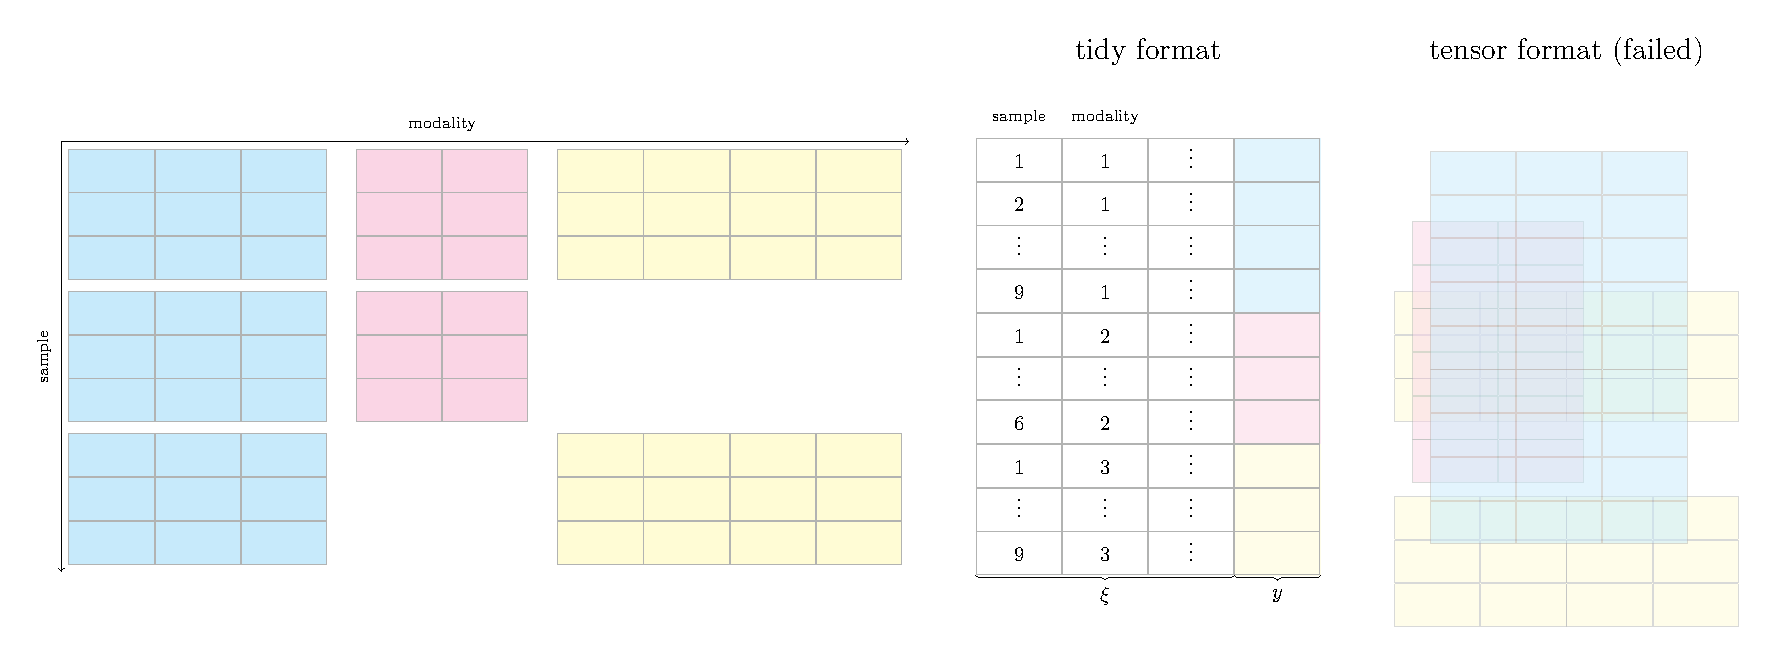
\includegraphics[width=0.95\textwidth]{img/mosaic}
\end{figure}
\begin{itemize}
\item semi-paired なデータが多い
\item モダリティごとに分布が変わる
\end{itemize}
}
\frame{
\frametitle{切断, Rectified, 離散化}
\begin{figure}
\centering
\begin{tabular}{c|cc}
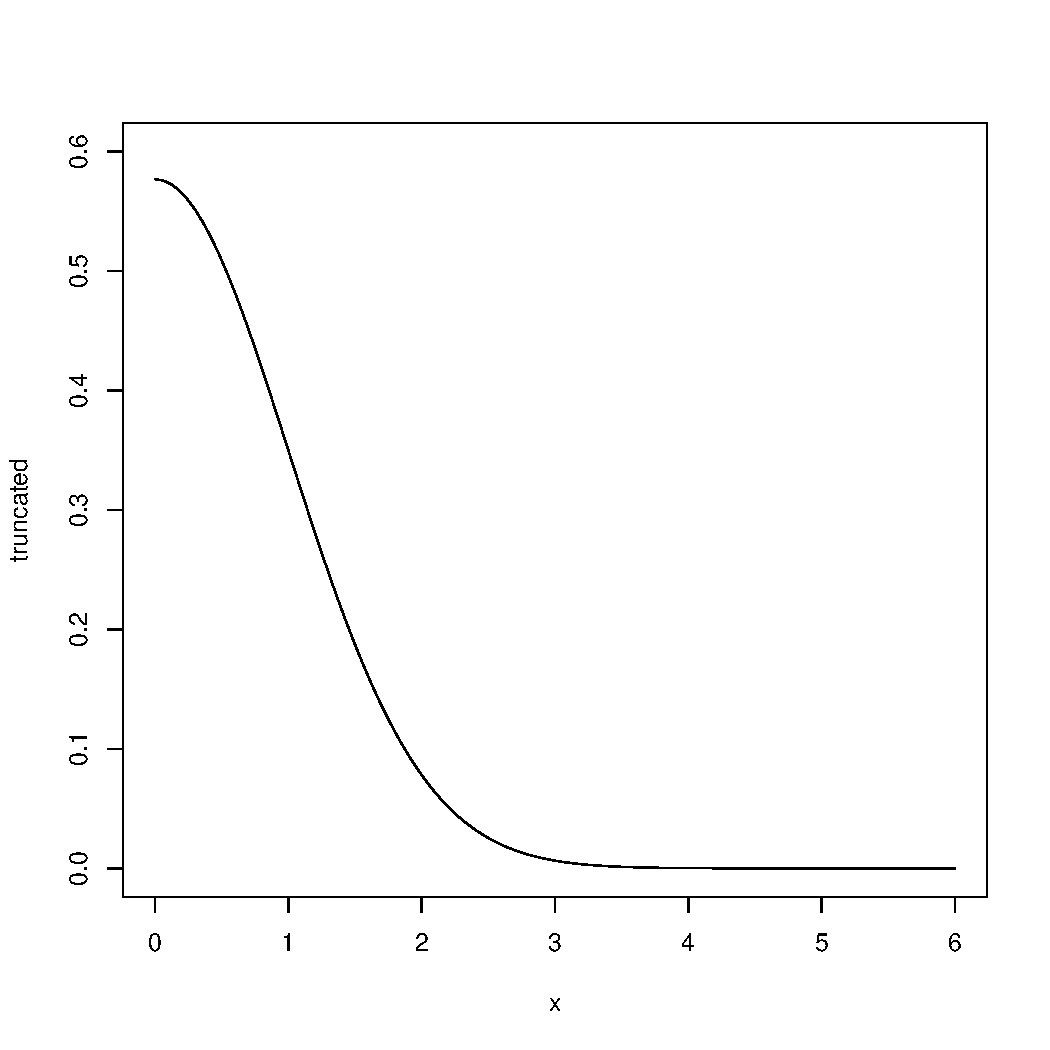
\includegraphics[width=0.3\textwidth]{img/norm_truncated} &
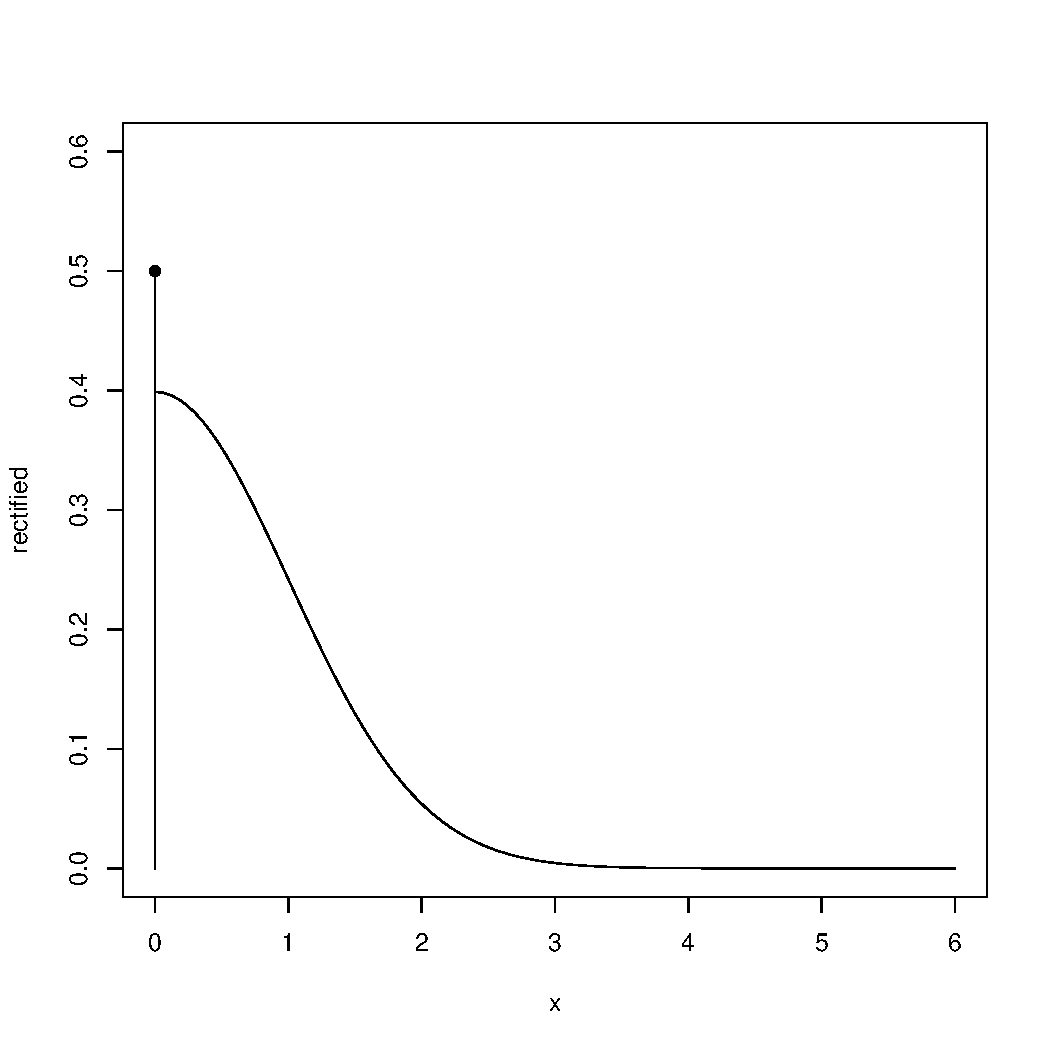
\includegraphics[width=0.3\textwidth]{img/norm_rectified} &
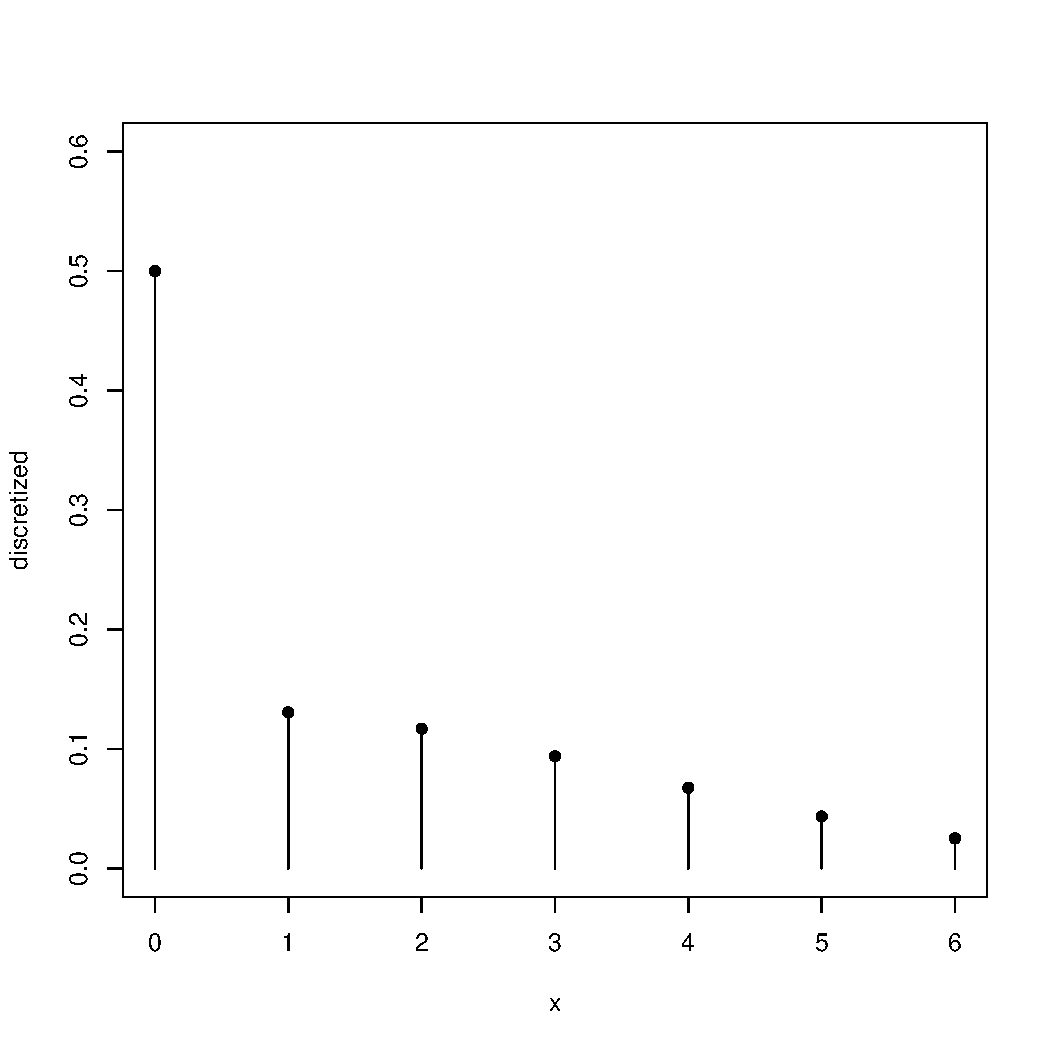
\includegraphics[width=0.3\textwidth]{img/norm_discretized}
\end{tabular}
\caption{\structure{left:} 潜在変数の事前分布. \structure{right:} 観測されるデータのモデル. 一点0で確率を持つ(eg. 重さ, 計数)}
\end{figure}
}
\frame{
data: $Y=(y_{ijk})$

$y=(y_n) = \operatorname{vec}(Y)$ as given . 

Let the $m$-th subscript of $y_{ijk}$ be $\xi_m$.
Canonical decomposition and parallel factor analysis (also known as CP decomposition) seeks matrices $v^{(m)}$ such that
\begin{equation*}
y_{ijk} \approx \sum_{l}v_{il}^{(1)} v_{jl}^{(2)} v_{kl}^{(3)}. 
\end{equation*}
This equation can be represented as follows:
\begin{equation}
y_{n} \approx \sum_{l}\prod_{d=1}^D v_{dr}^{x_{nd}} \label{eq_approx}
\end{equation}
where
\begin{align*}
V=(v_{dl})=\begin{pmatrix}
v^{(1)}\\
v^{(2)}\\
v^{(3)}
\end{pmatrix}
\end{align*}
}
\frame{
\frametitle{モデル0}

式1 $y_{n} \approx \sum_{l} \prod_{d=1}^D v_{dl}^{x_{nd}}$; はややあいまい

次のように書き直す:
\begin{align}
y_n & \sim \normal\left(y_n \mid \sum_{l=1}^L \prod_{d=1}^D v_{dl}^{x_{nd}}, \lambda^{-1}\right) \label{eq_mod1}\\
v_{dl} & \sim \normal(v_{dl} | 0,\tau^{-1}) \label{eq_prior1}\\
\lambda & \sim \gam(\lambda | a,b) \nonumber
\end{align}

このモデルを修正・拡張する:
\begin{itemize}
\item 非負制約(解釈性)
\item 分布を変える(マルチオミクス)
\end{itemize}
}
\frame{
\frametitle{事前分布:非負制約}
}
\frame{
\frametitle{中間変数}
}
\end{document}  